DPC++提供了一组关于各种数据类型的丰富的SYCL内置函数。这些内置函数可以在主机和设备上的sycl命名空间中使用,基于编译器选项(例如DPC++编译器提供的-mfma、- fast-math和-ffp-contract=fast)对目标设备提供低、中、高精度支持。主机和设备上的这些内置功能可以分为以下几类:\par

\begin{itemize}
	\item 浮点数学函数asin、acos、log、sqrt、floor等,如图18-2。
	\item 整数函数:abs、max、min等,如图18-3。
	\item 常用函数:clamp, smoothstep等,如图18-4。
	\item 几何函数:cross, dot, distance等,如图18-5。
	\item 关系函数:isequal, isless, isfinite等,如图18-6。
\end{itemize}

如果一个函数是由C++ std库提供的(如图18-8所示),以及一个SYCL内置函数,则DPC++开发者可以使用其中任何一个。图18-1展示了C++ std::log函数和SYCL内置的用于主机和设备的SYCL::log函数,这两个函数产生相同的结果。本例中,内置关系函数sycl::isequal用于比较std:log和sycl:log的结果。\par

\hspace*{\fill} \par %插入空行
图18-1 使用std::log和sycl::log
\begin{lstlisting}[caption={}]
constexpr int size = 9;
std::array<double, size> A;
std::array<double, size> B;

bool pass = true;

for (int i = 0; i < size; ++i) { A[i] = i; B[i] = i; }

queue Q;
range sz{size};

buffer<double> bufA(A);
buffer<double> bufB(B);
buffer<bool> bufP(&pass, 1);

Q.submit([&](handler &h) {
	accessor accA{ bufA, h};
	accessor accB{ bufB, h};
	accessor accP{ bufP, h};
	
	h.parallel_for(size, [=](id<1> idx) {
		accA[idx] = std::log(accA[idx]);
		accB[idx] = sycl::log(accB[idx]);
		if (!sycl::isequal( accA[idx], accB[idx]) ) {
			accP[0] = false;
		}
	});
});
\end{lstlisting}

除了SYCL中支持的数据类型外,DPC++设备库还提供了对std:complex数据类型,以及C++ std库中定义的相应数学函数的支持\par

\hspace*{\fill} \par %插入空行
\textbf{内置函数中使用sycl::前缀}

调用SYCL内置函数时,应该在名称前添加显式的sycl::。对于当前的SYCL规范,即使使用了“using namespace sycl;”,也不能保证只调用sqrt()就能调用所有实现上的内置SYCL。\par

\begin{tcolorbox}[colback=red!5!white,colframe=red!75!black]
调用SYCL内置函数时,应该始终在内置名称前面显式地加上sycl::。不遵循此建议可能会导致奇怪和不可移植的结果。
\end{tcolorbox}

如果在应用程序中,内置函数的名称与非模板函数冲突,在许多实现中(包括DPC++),我们的内置函数将占上风,这是因为C++的重载解析规则更喜欢非模板函数而不是模板函数。然而,如果代码有一个与内置名称相同的函数名,那么为了保证可移植性,就是避免使用命名空间sycl,或者确保没有实际冲突发生。否则,一些SYCL编译器将由于其实现中无法解决的冲突而拒绝编译代码。这样的冲突不会停止。因此,今天编译的代码,可以安全地忽略未来出现问题的可能性。\par

\hspace*{\fill} \par %插入空行
图18-2 内置数学函数
\begin{center}
	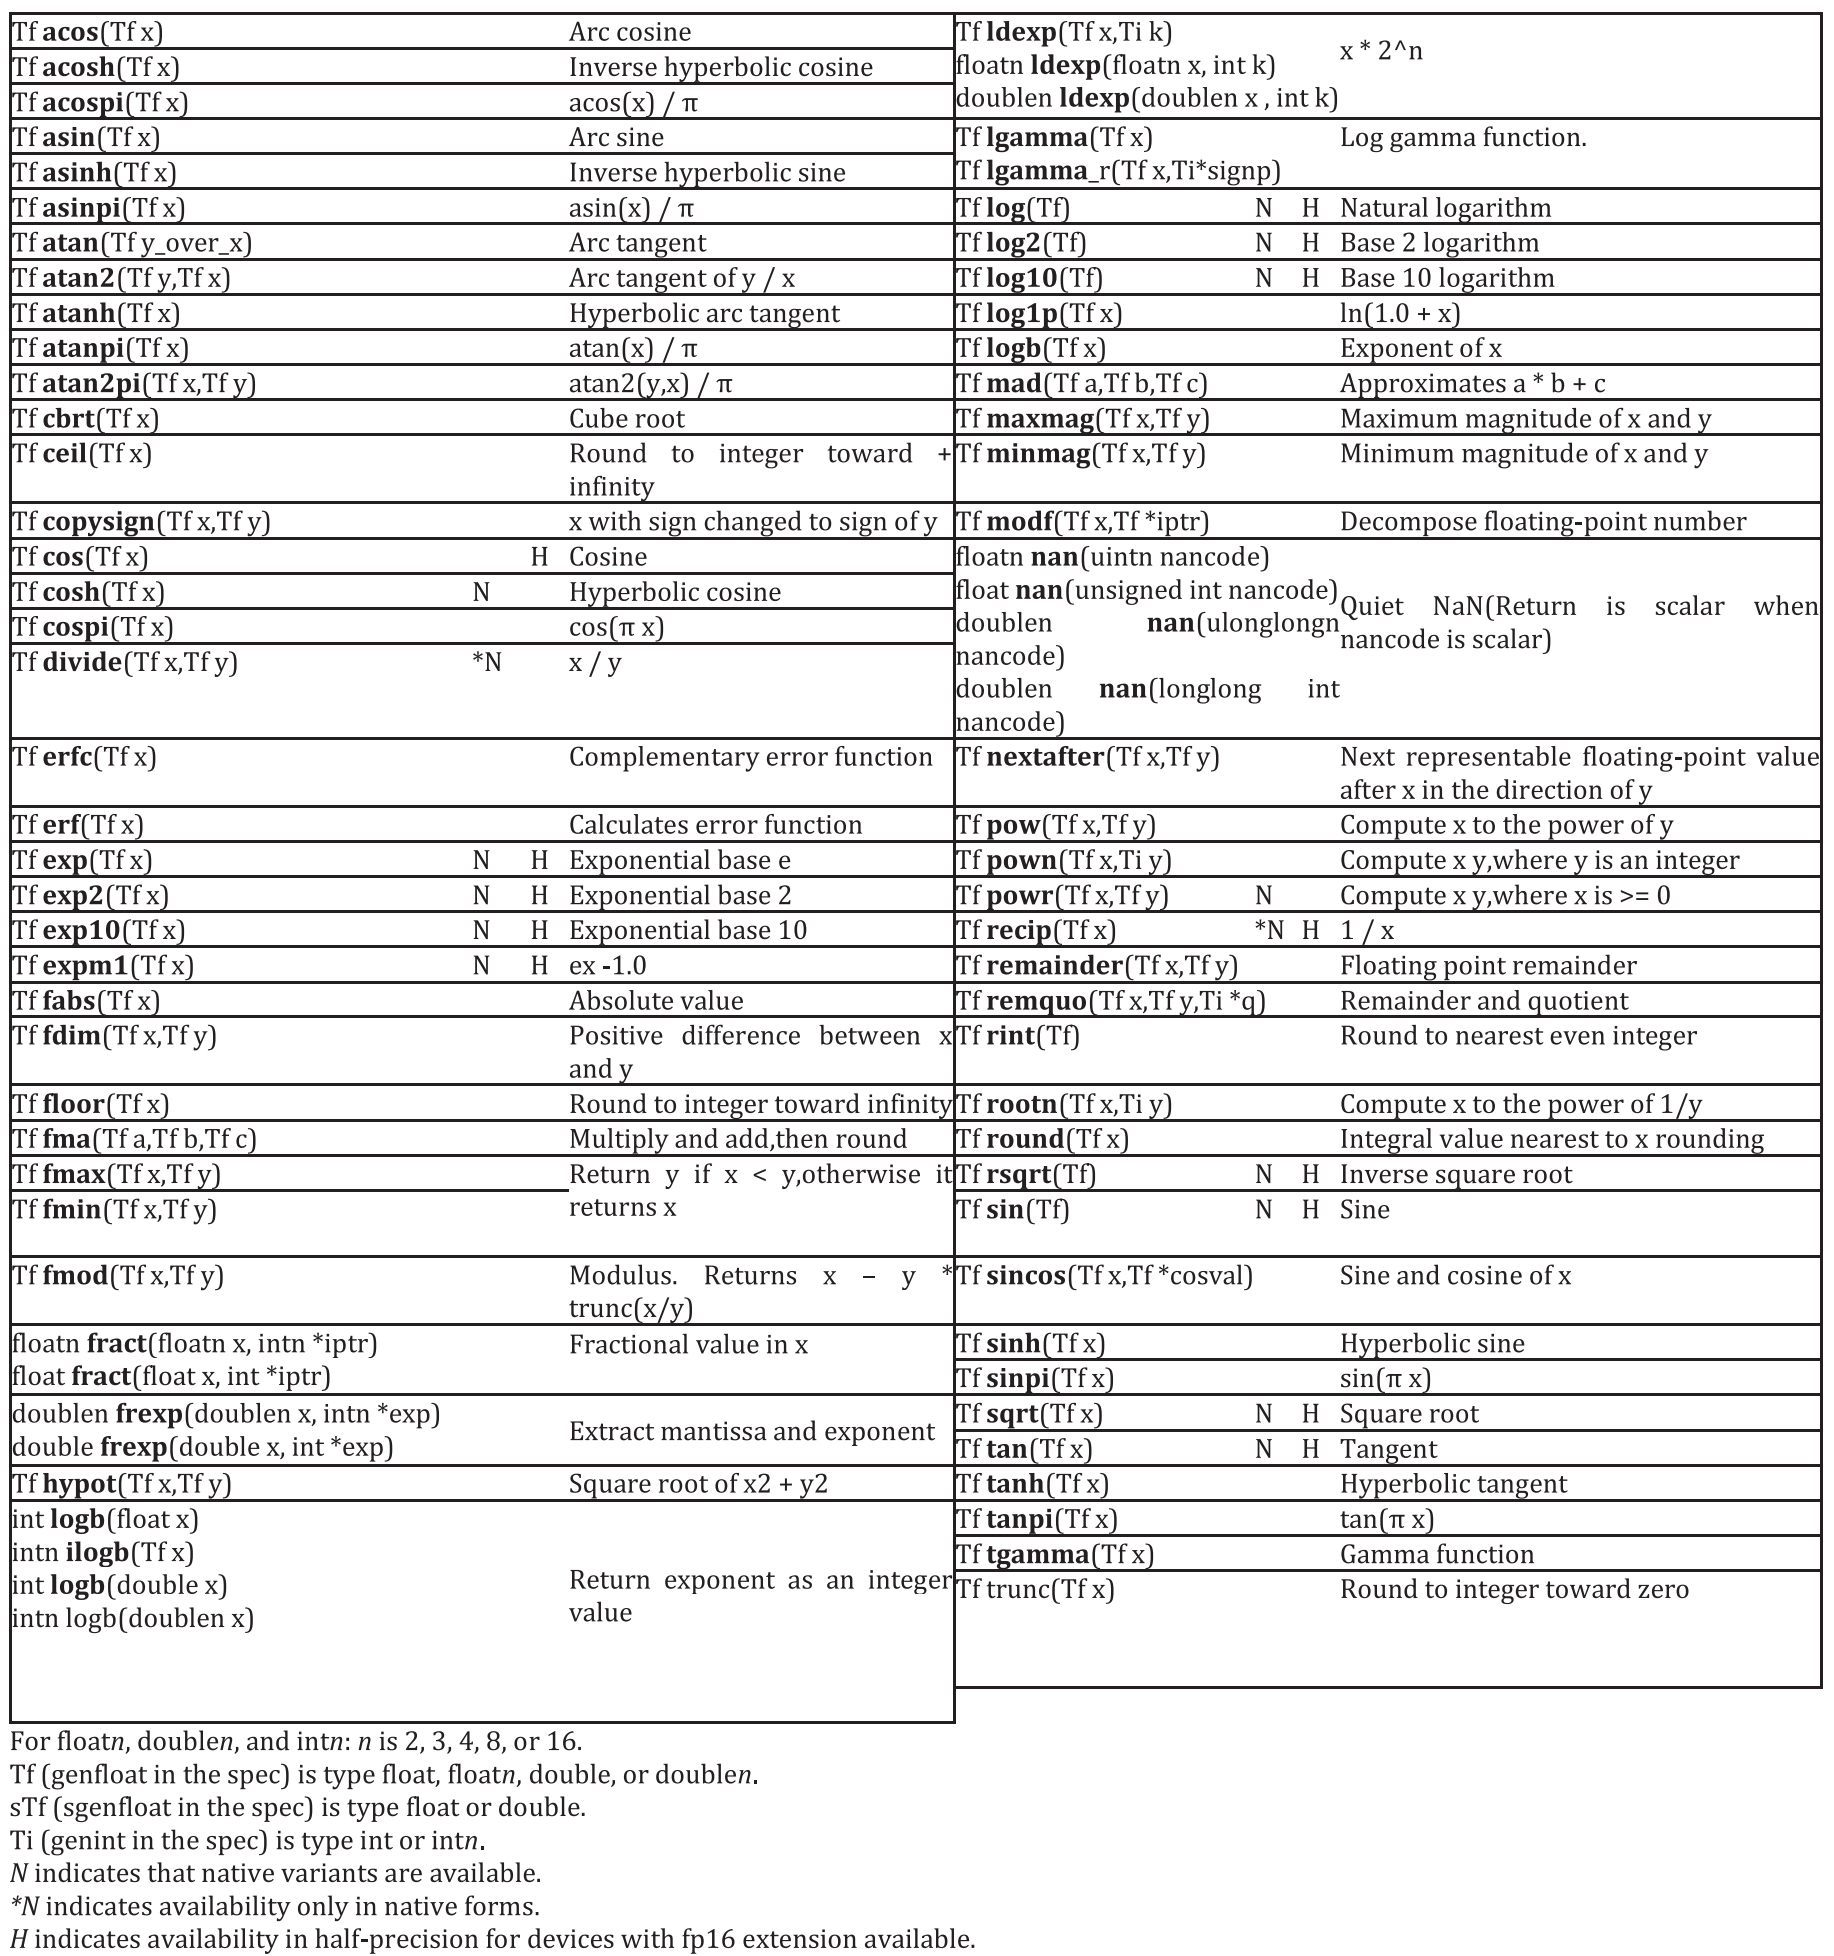
\includegraphics[width=1.0\textwidth]{content/chapter-18/images/2}
\end{center}

\hspace*{\fill} \par %插入空行
图18-3 内置整数函数
\begin{center}
	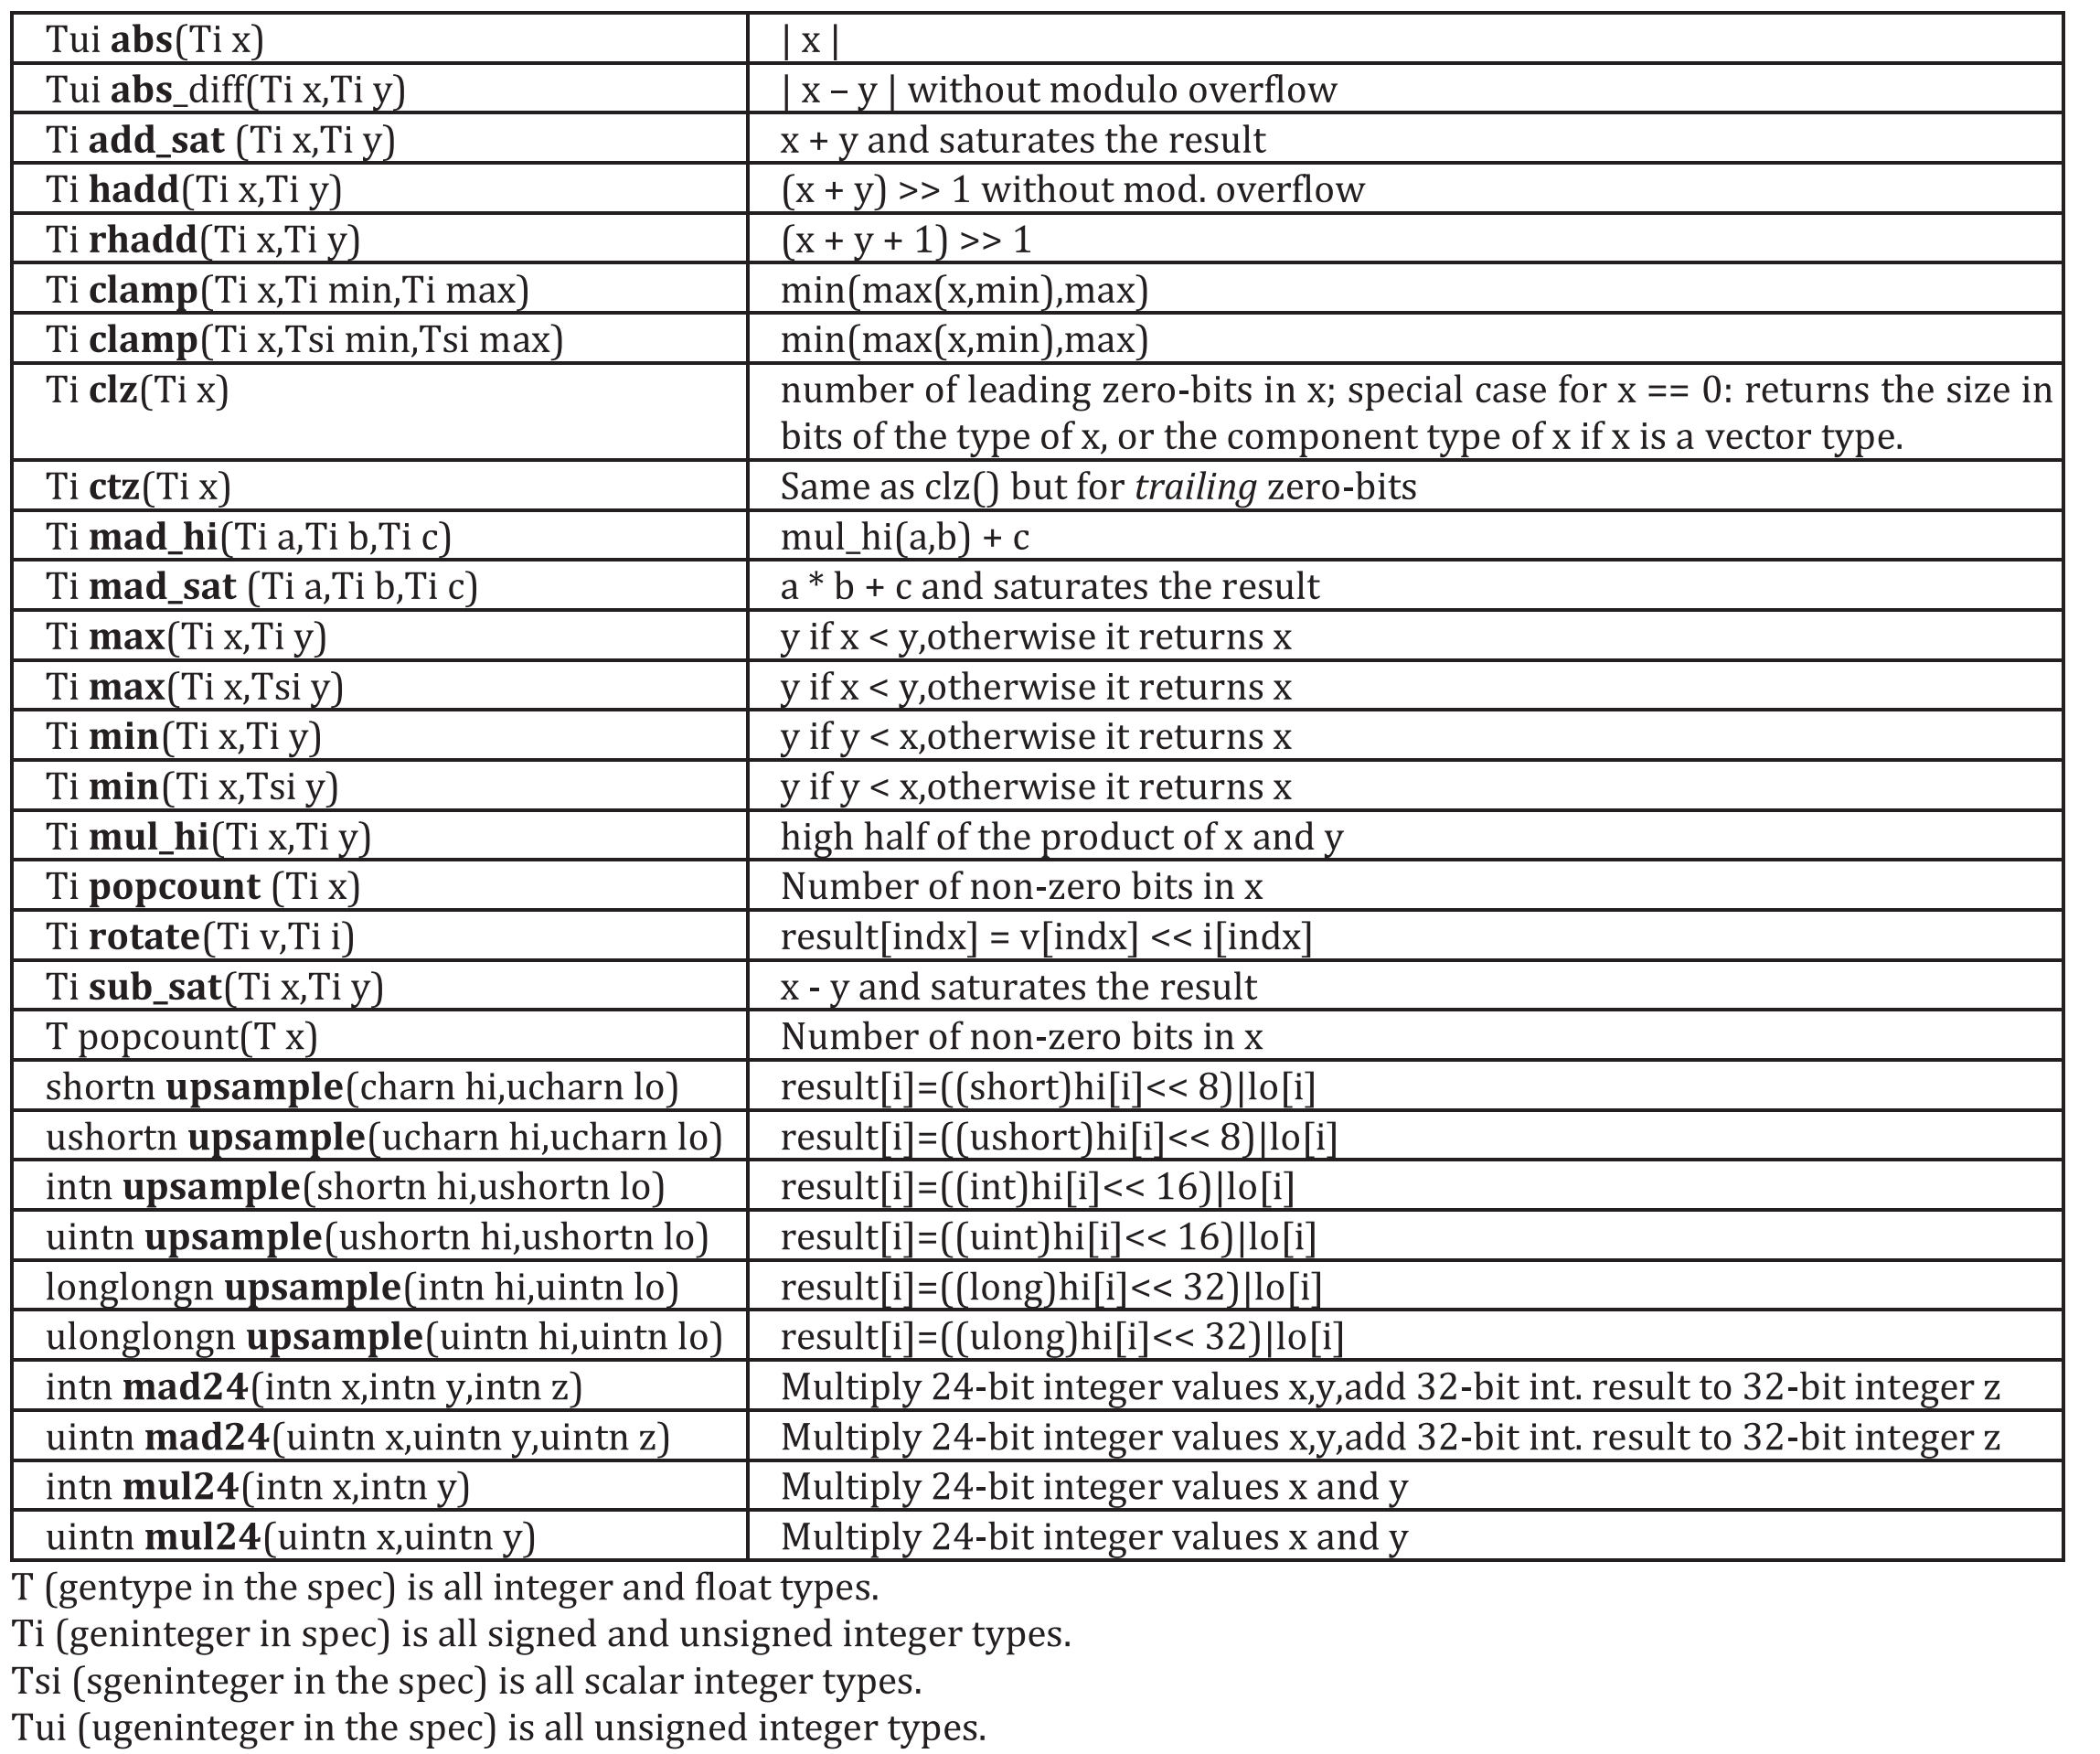
\includegraphics[width=1.0\textwidth]{content/chapter-18/images/3}
\end{center}

\hspace*{\fill} \par %插入空行
图18-4 内置通用函数
\begin{center}
	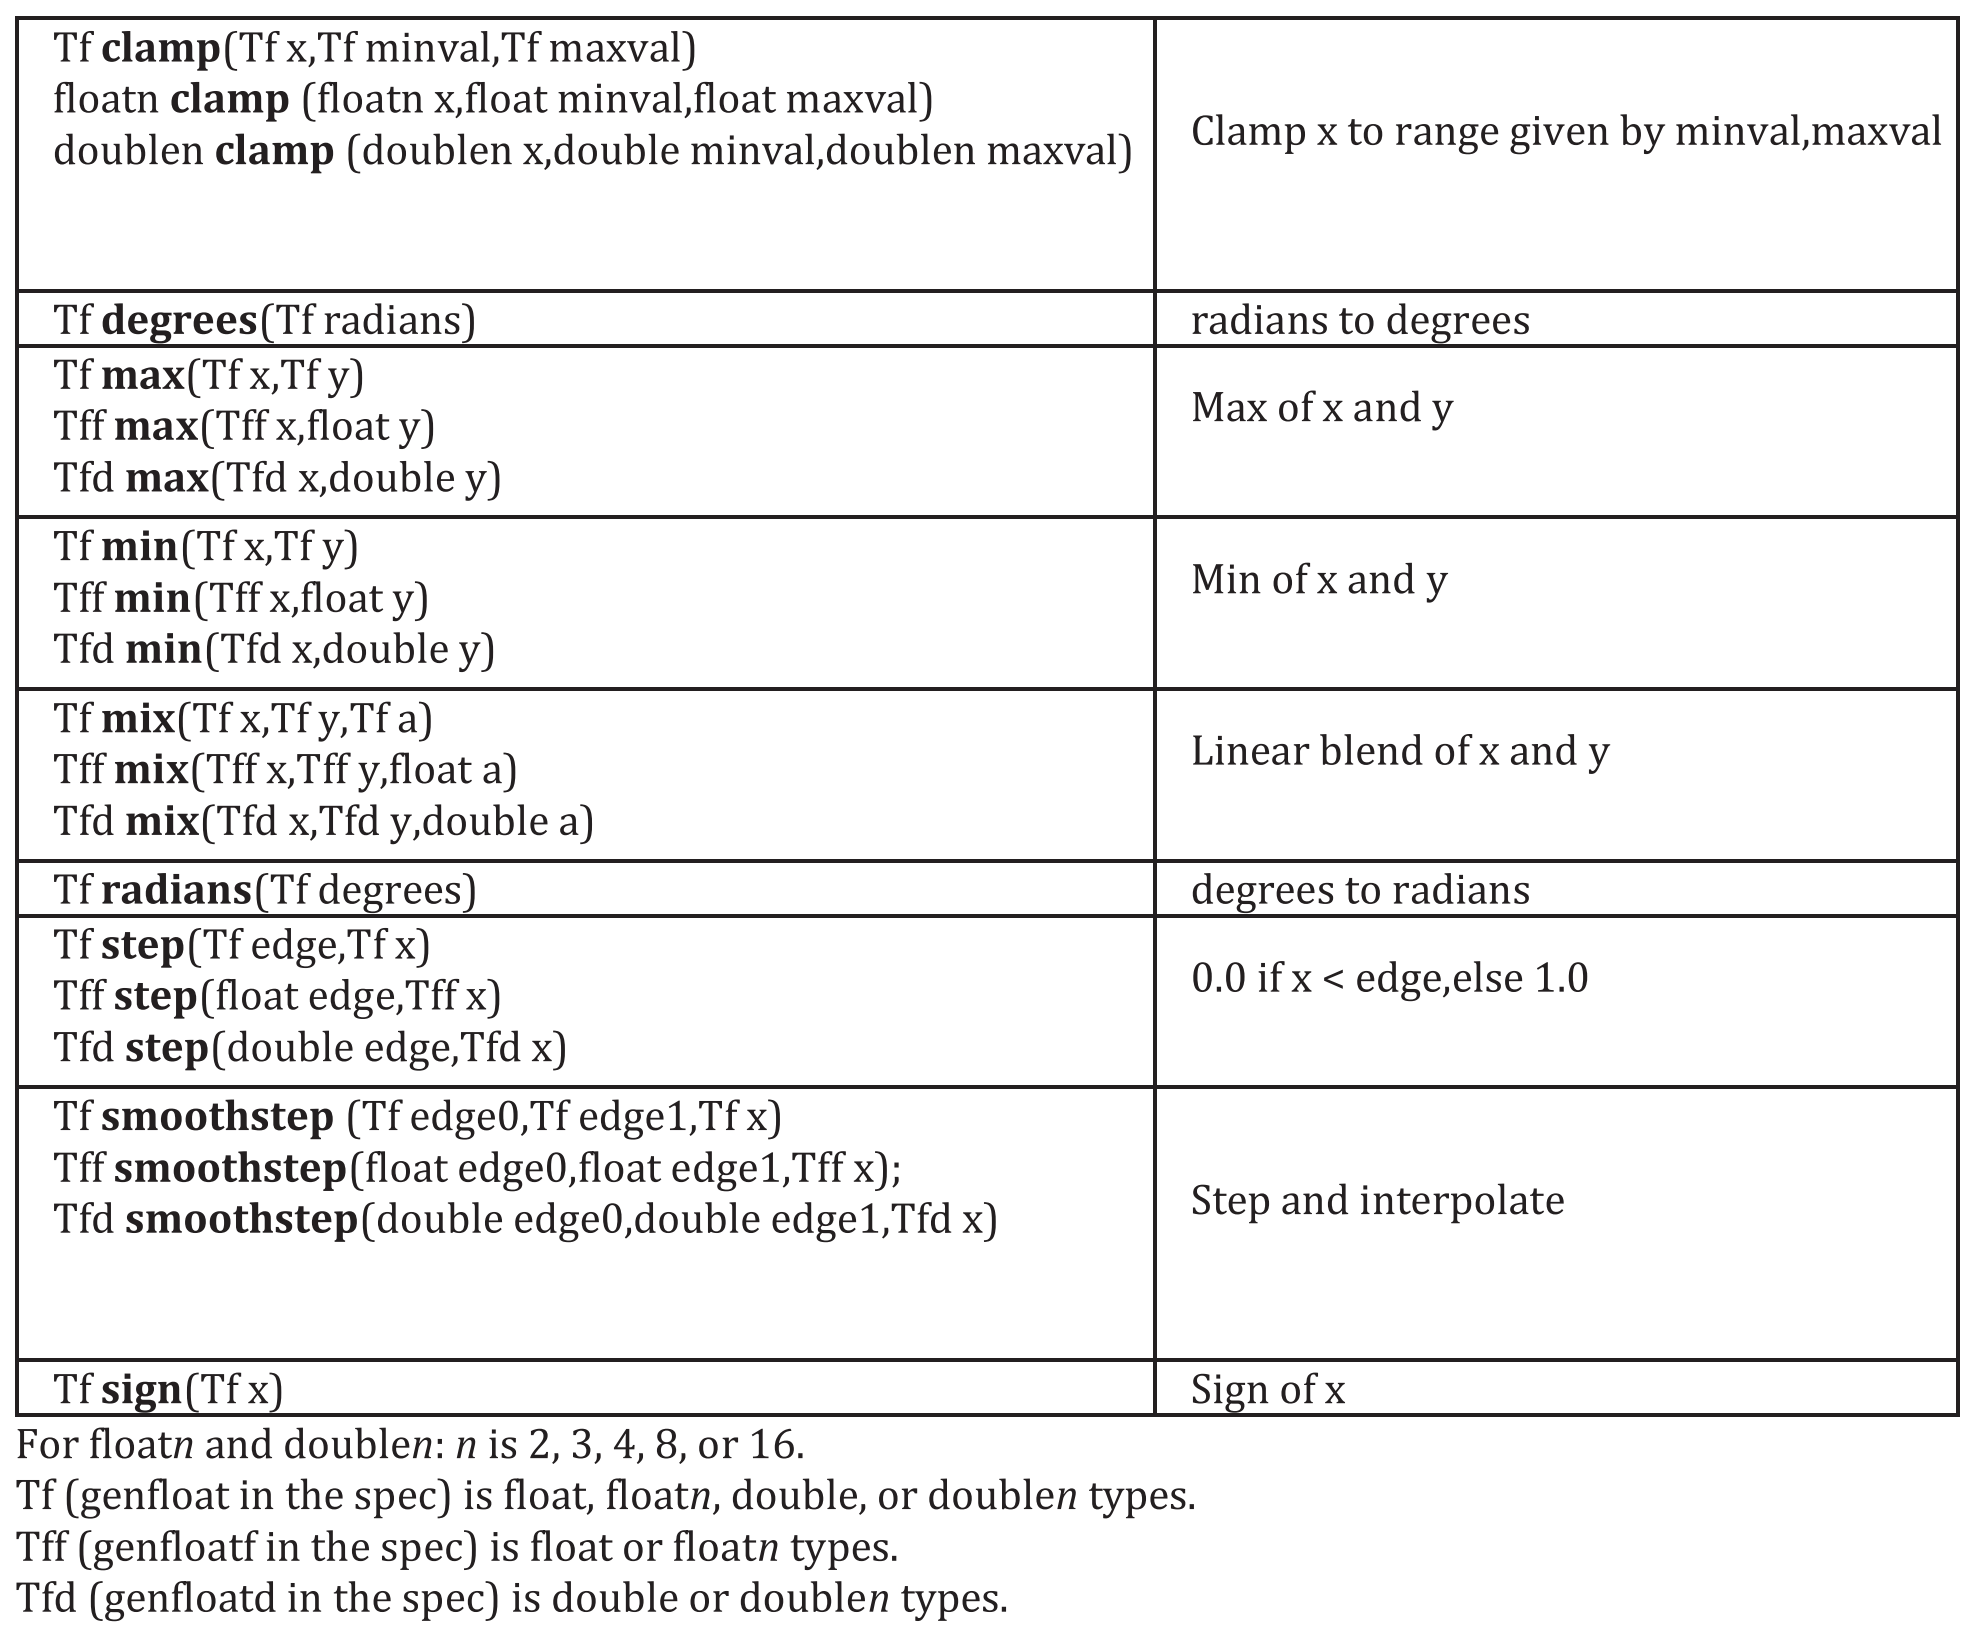
\includegraphics[width=1.0\textwidth]{content/chapter-18/images/4}
\end{center}

\hspace*{\fill} \par %插入空行
图18-5 内置几何函数
\begin{center}
	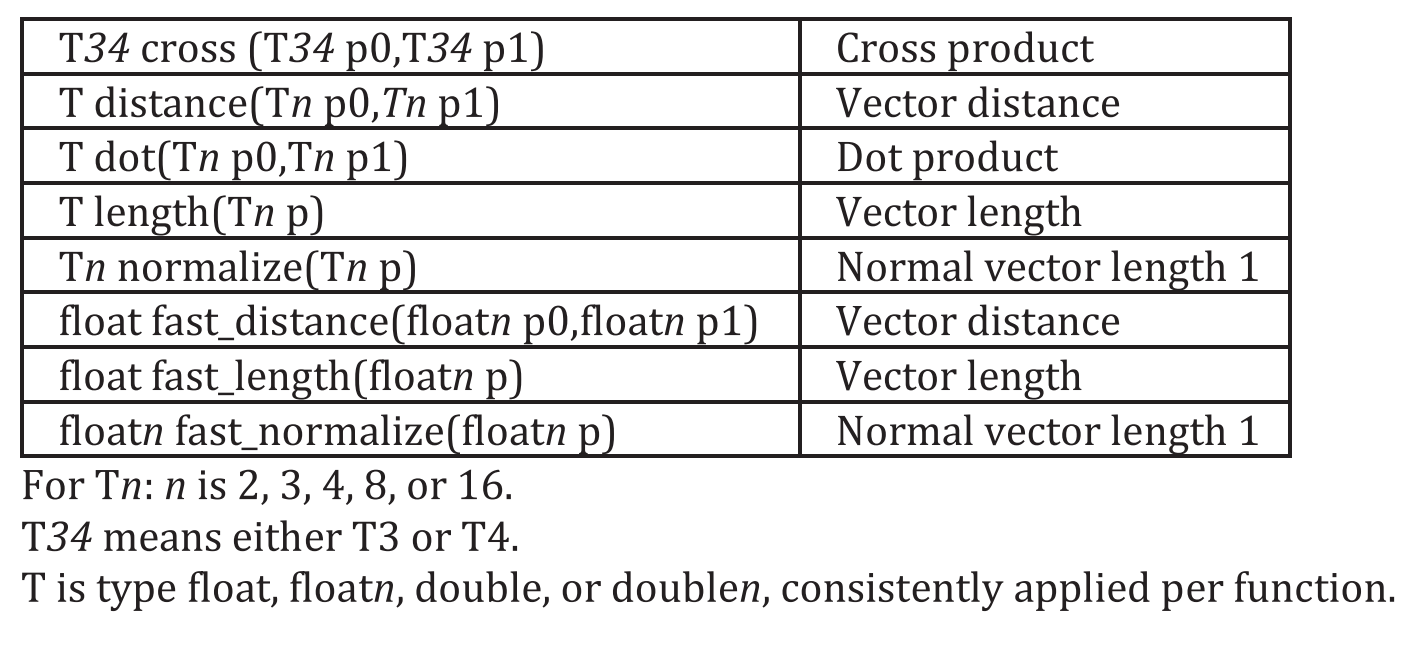
\includegraphics[width=1.0\textwidth]{content/chapter-18/images/5}
\end{center}

\hspace*{\fill} \par %插入空行
图18-6 内置关系函数
\begin{center}
	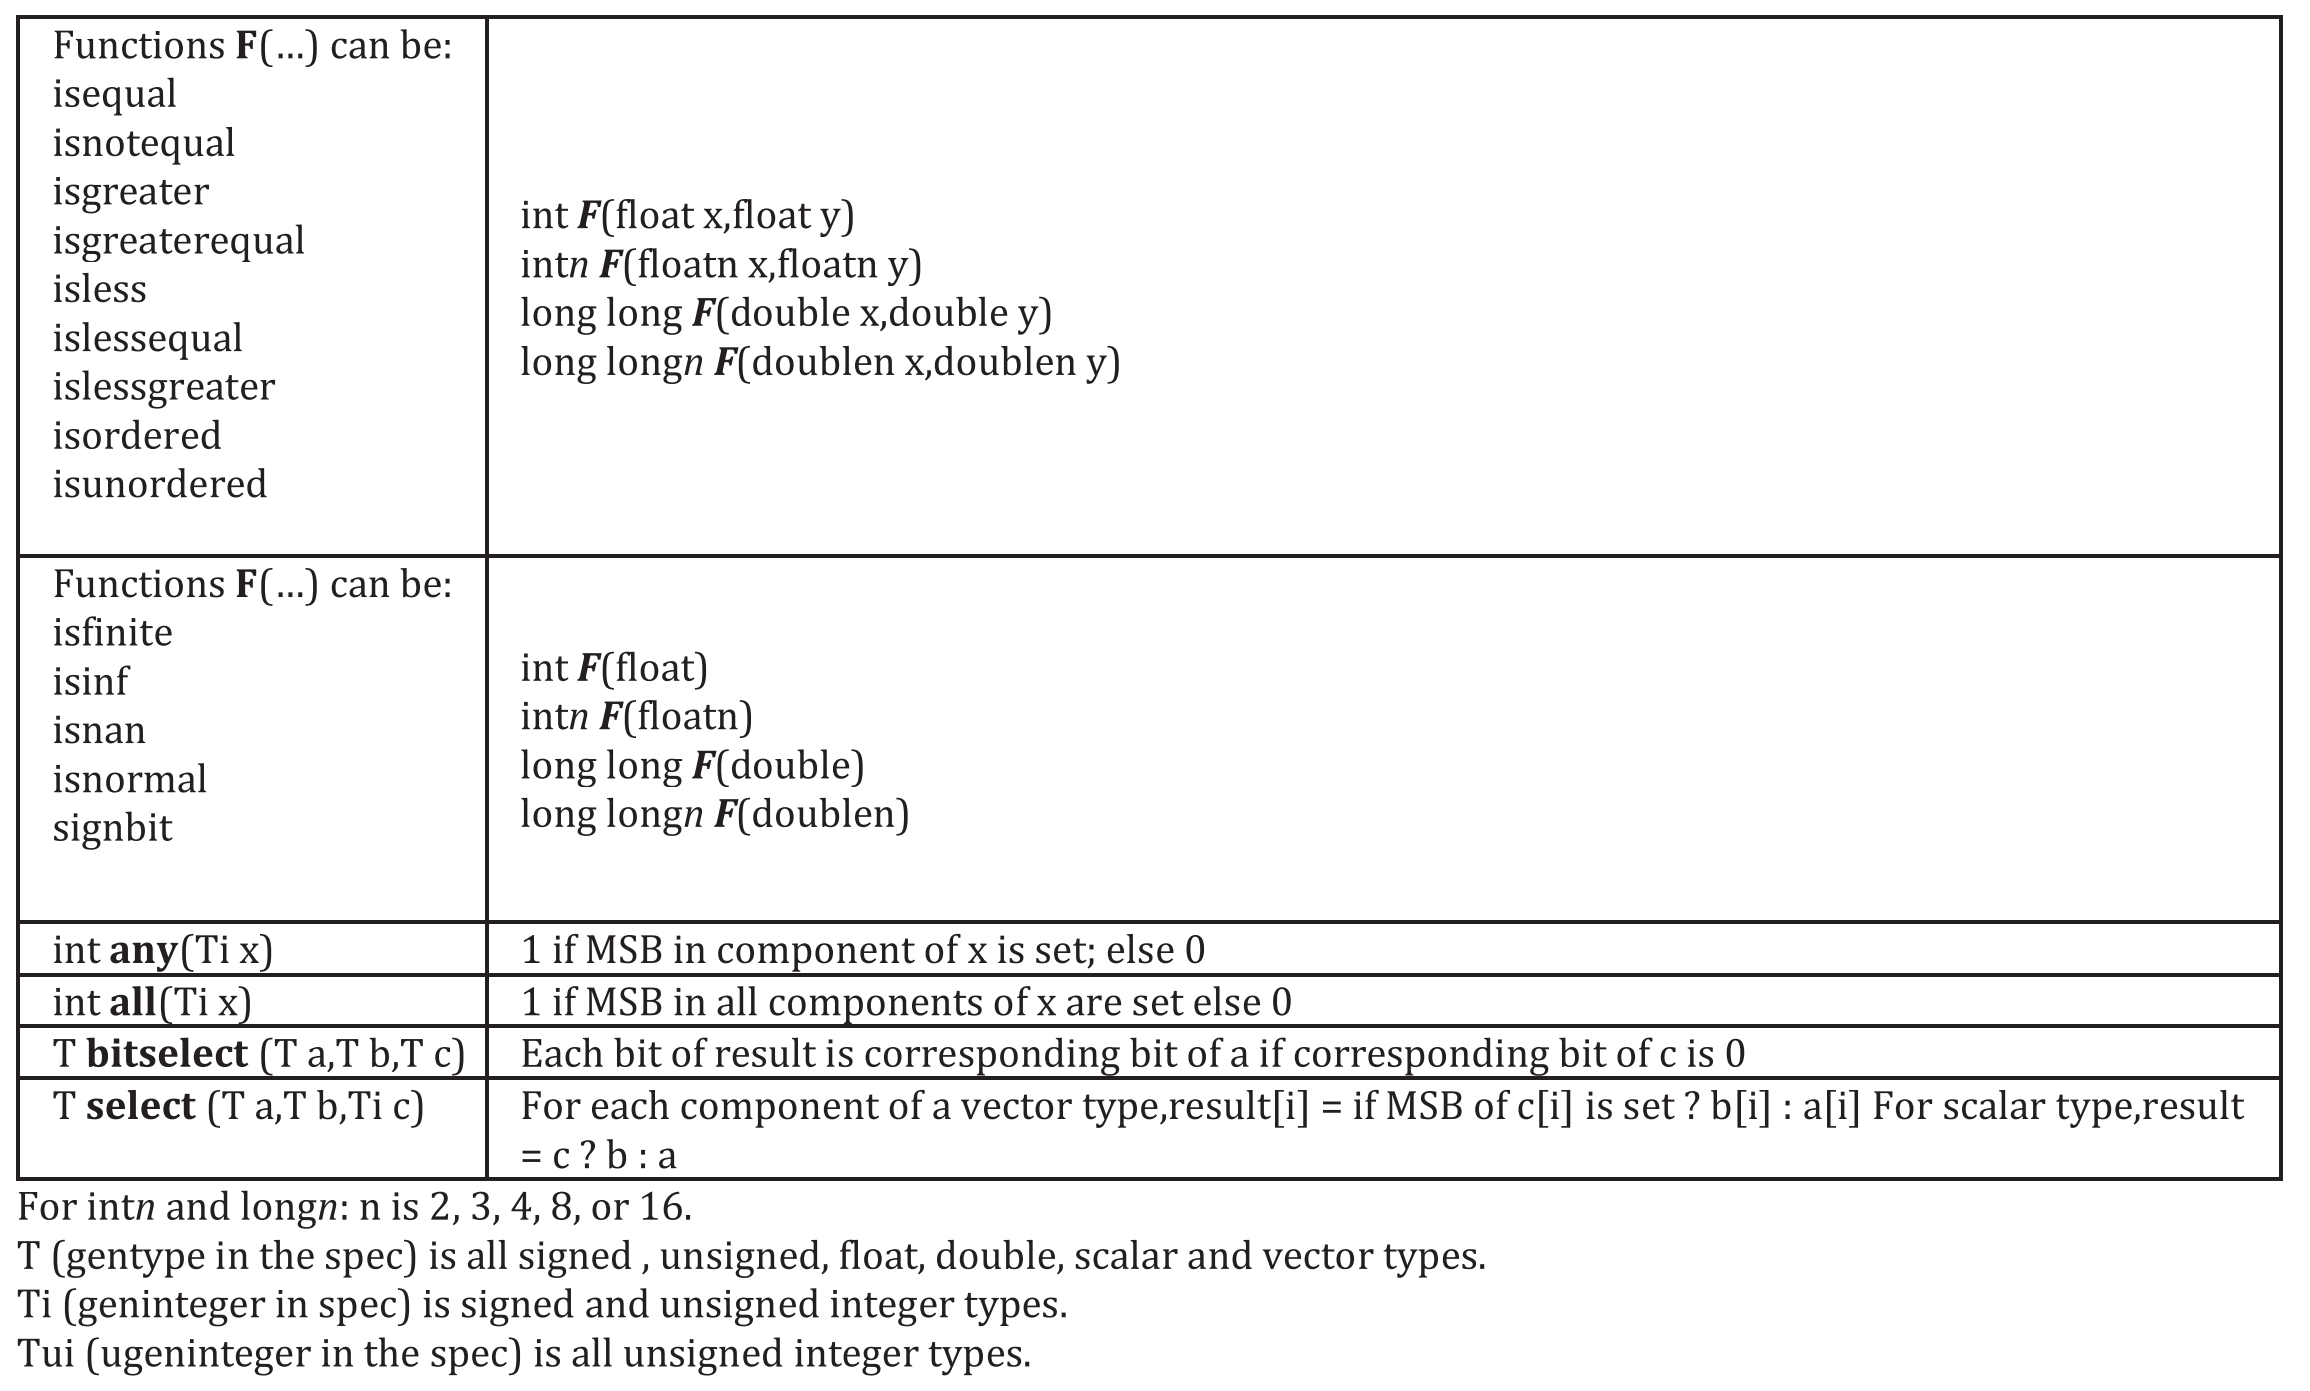
\includegraphics[width=1.0\textwidth]{content/chapter-18/images/6}
\end{center}




























































